%==============================================================================
% Capítulo 8: Resultados
%==============================================================================
\section{Resultados}\label{sec:resultados}

Este capítulo presenta los resultados de la validación experimental en cuatro dimensiones: tiempos de registro, desempeño de clasificación, reducción de la intervención humana y análisis cualitativo de errores.

\subsection{Comparación de tiempos de registro}\label{subsec:comparacion-tiempos}

La comparación de los tiempos de registro entre el flujo manual y el flujo automatizado se sintetiza en la Tabla~\ref{tab:tiempos}. La media aritmética del tiempo manual sobre los 200 casos del corpus fue de 61,6~s (mediana de 50,0~s), con un desvío estándar de 44,9~s y un rango entre 10 y 300~s. Este valor, respaldado por la planilla de cronometraje descrita en la \autoref{subsec:diseno-experimental}, corresponde a la medición experimental incidente por incidente y reemplaza a la estimación preliminar de 2 minutos con 45 segundos citada en la \autoref{subsec:planteamiento-problema}, obtenida sin cronometraje individual. La media del flujo automatizado fue de 17,76~s (mediana de 17,47~s), con un desvío estándar de 13,48~s y un rango entre 0,525 y 65,834~s. La reducción relativa de la media de tiempo alcanzó el 71,2~\%.

\begin{table}[htbp]
\centering
\caption{Estadísticos descriptivos de los tiempos de registro por flujo (\(n = 200\))}
\label{tab:tiempos}
\small
\begin{tabular}{@{}>{\raggedright\arraybackslash}p{4.0cm} p{3.5cm} p{3.5cm} p{2.5cm}@{}}
\toprule
\textbf{Estadístico} & \textbf{Flujo manual} & \textbf{Flujo automatizado} & \textbf{Reducción} \\
\midrule
Media aritmética (s)      & 61,6   & 17,76   & 71,2~\% \\
Mediana (s)               & 50,0   & 17,47   & 65,1~\% \\
Desvío estándar (s)       & 44,9   & 13,48   & --- \\
Mínimo (s)                & 10     & 0,525   & --- \\
Máximo (s)                & 300    & 65,834  & --- \\
\bottomrule
\end{tabular}
\par\smallskip
{\footnotesize\textit{Fuente:} elaboración propia a partir del corpus de validación (\(n = 200\)).\par}
\end{table}

El tiempo automatizado de registro desagregado por canal de origen se presenta en la Tabla~\ref{tab:tiempos-canal}. El canal telefónico incorpora, además de la latencia de procesamiento, la duración de la llamada grabada; como la grabación esta acotada a un máximo de 45~s (véase la \autoref{subsec:metricas-instrumentos}), su valor constituye una cota inferior de la duración real de la llamada.

\begin{table}[htbp]
\centering
\caption{Tiempo automatizado de registro por canal de origen (\(n = 200\))}
\label{tab:tiempos-canal}
\small
\begin{tabular}{@{}p{6.0cm} c c c@{}}
\toprule
\textbf{Canal de origen} & \textbf{Casos} & \textbf{Media (s)} & \textbf{Mediana (s)} \\
\midrule
Llamada telefónica (cota inferior) & 81 & 20,09 & 18,70 \\
Correo electrónico                 & 66 & 27,65 & 25,82 \\
Formulario web                     & 53 & 1,88  & 1,26  \\
\midrule
\textbf{Global}                    & \textbf{200} & \textbf{17,76} & \textbf{17,47} \\
\bottomrule
\end{tabular}
\par\smallskip
{\footnotesize\textit{Fuente:} elaboración propia a partir del corpus de validación (\(n = 200\)).\par}
\end{table}

La prueba de Wilcoxon de rangos con signo aplicada sobre las mediciones pareadas \parencite{Virtanen2020_scipy} arrojó un estadístico de contraste \(W = \min(T^{+}, T^{-}) = 363\), con una suma de rangos positivos \(T^{+} = 19.737\), una suma de rangos negativos \(T^{-} = 363\) y \(n = 200\) pares válidos, junto con un valor \(p = 3{,}08 \times 10^{-32}\), lo que permite rechazar la hipótesis nula de igualdad de medianas con un nivel de confianza superior al 99,9~\%. El estadístico refleja que en 188 de los 200 pares el flujo automatizado fue más veloz que el manual; en los 12 pares restantes (6,0~\%) el flujo automatizado no fue más rápido, resultado coherente con la diferencia de aproximadamente 32,5~s entre medianas. La prueba se eligió por el rechazo de la normalidad en los tres conjuntos de tiempos (\autoref{subsec:analisis-estadistico}).

Para cuantificar la magnitud práctica de la diferencia, se calculó el coeficiente \(r\) de correlación rank-biserial a partir de los dos estadísticos de rango:
\[
r = \frac{T^{+} - T^{-}}{n(n+1)/2} = \frac{19.737 - 363}{200 \cdot 201 / 2} = \frac{19.374}{20.100} = 0{,}9639
\]
El valor obtenido (\(r = 0{,}9639\)) corresponde a un tamaño del efecto muy alto. La diferencia observada es, por tanto, estadísticamente significativa y, dada su magnitud absoluta, relativa y el tamaño del efecto reportado, también prácticamente relevante para la operación.

Cabe señalar que el tiempo manual se registró con redondeo hacia arriba (véase la \autoref{subsec:diseno-experimental}), un sesgo de medición sistemático que infla la línea base manual. Por ese motivo la reducción del 71,2~\% debe leerse como cota superior. Un análisis de sensibilidad que descuenta 5~s y 10~s a cada medición manual reduce la media manual a 56,6~s y 51,6~s, respectivamente, y sitúa la reducción en el 68,6~\% y en el 65,6~\% como cota inferior conservadora. Aun en el escenario más desfavorable la reducción de tiempo permanece sustancial y estadísticamente significativa (\(p = 1{,}8 \times 10^{-26}\), \(r = 0{,}8683\)).

\begin{figure}[htbp]
\centering
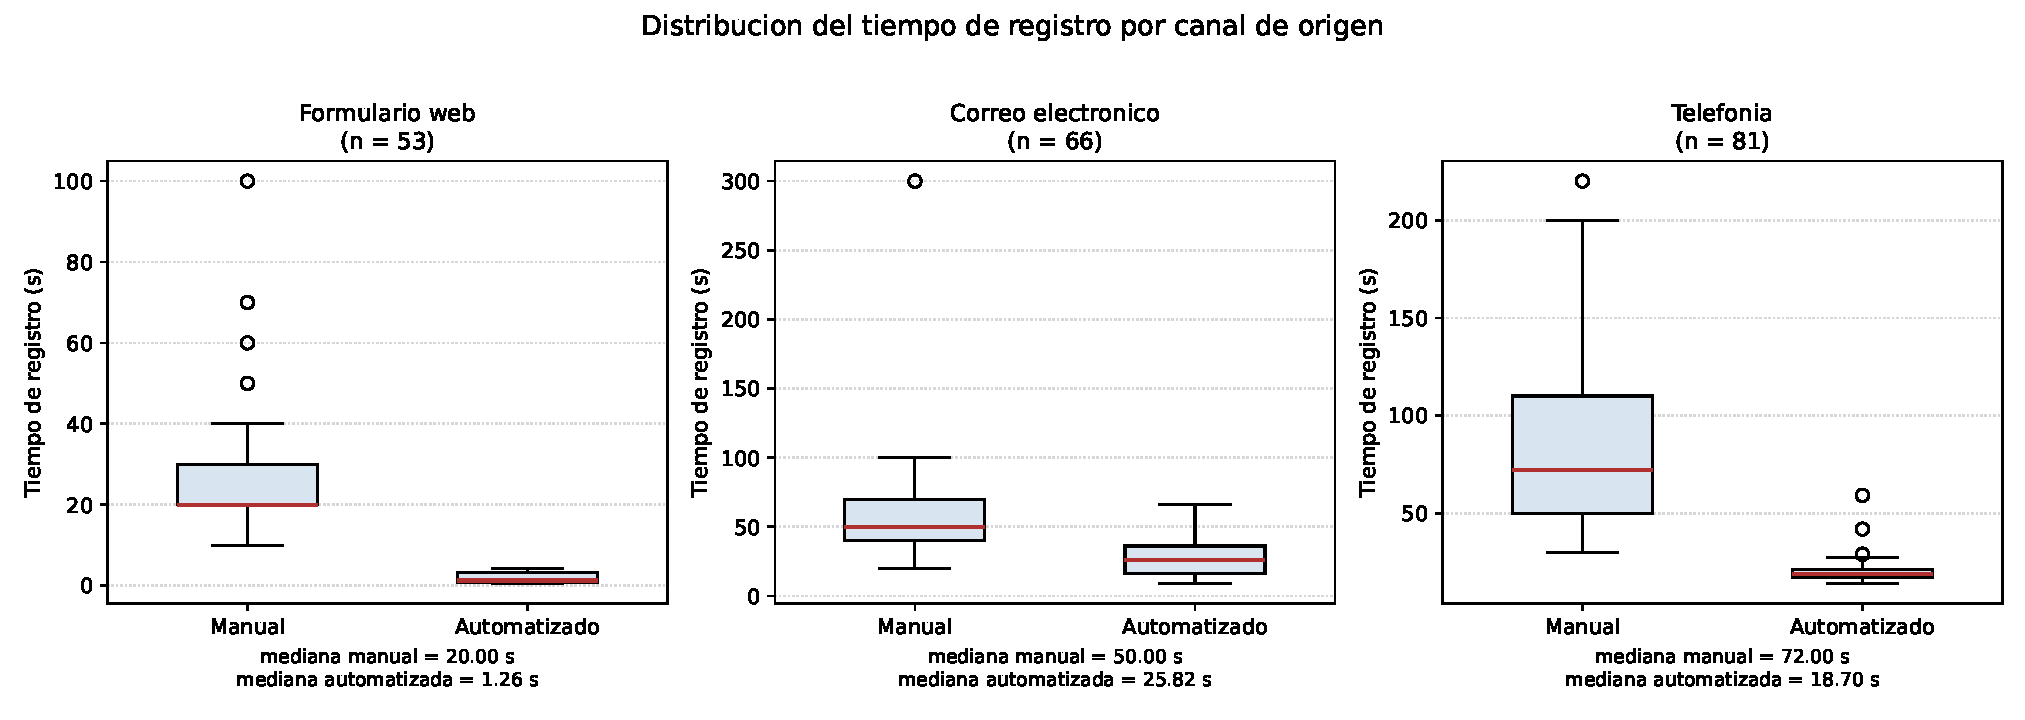
\includegraphics[width=\textwidth]{boxplot_tiempos}
\caption{Distribución del tiempo de registro por canal de origen (manual frente a automatizado). El panel de telefonía incorpora la duración de la llamada grabada.}
\label{fig:boxplot_tiempos}
\end{figure}

\subsection{Matriz de confusión y métricas de clasificación}\label{subsec:matriz-metricas}

La evaluación de clasificación se realizó sobre el corpus real de 200 casos pseudonimizados, cuya distribución por sector y por canal se describe en la \autoref{subsec:poblacion-muestra-corpus}.

La matriz de confusión obtenida se presenta en la Tabla~\ref{tab:matriz} y en la Figura~\ref{fig:matriz_confusion}. La exactitud estricta resultante asciende al 73,5~\% (147 casos correctos sobre 200).

\begin{table}[htbp]
\centering
\caption{Matriz de confusión del clasificador automático (\(n = 200\)). Filas: sector asignado; columnas: sector predicho principal.}
\label{tab:matriz}
\small
\setlength{\tabcolsep}{4pt}
\begin{tabular}{@{}>{\raggedright\arraybackslash}p{2.6cm} *{5}{>{\centering\arraybackslash}p{1.85cm}} >{\centering\arraybackslash}p{1.3cm}@{}}
\toprule
\textbf{Asignado \(\backslash\) Predicho} & \textbf{Seguridad Informatica} & \textbf{Soporte Tecnico Hardware} & \textbf{Soporte Tecnico Software} & \textbf{Bases de Datos} & \textbf{Sistemas} & \textbf{Total} \\
\midrule
Seguridad Informatica & 15 & 2 & 11 & 2 & 1 & \textbf{31} \\
Soporte Tecnico Hardware & 1 & \textbf{77} & 3 & 0 & 4 & \textbf{85} \\
Soporte Tecnico Software & 0 & 11 & \textbf{48} & 1 & 7 & \textbf{67} \\
Bases de Datos & 0 & 0 & 1 & 0 & 0 & \textbf{1} \\
Sistemas & 2 & 0 & 5 & 2 & \textbf{7} & \textbf{16} \\
\midrule
\textbf{Total} & \textbf{18} & \textbf{90} & \textbf{68} & \textbf{5} & \textbf{19} & \textbf{200} \\
\bottomrule
\end{tabular}
\par\smallskip
{\footnotesize\textit{Fuente:} elaboración propia a partir del corpus de validación (\(n = 200\)).\par}
\end{table}

\begin{figure}[htbp]
\centering
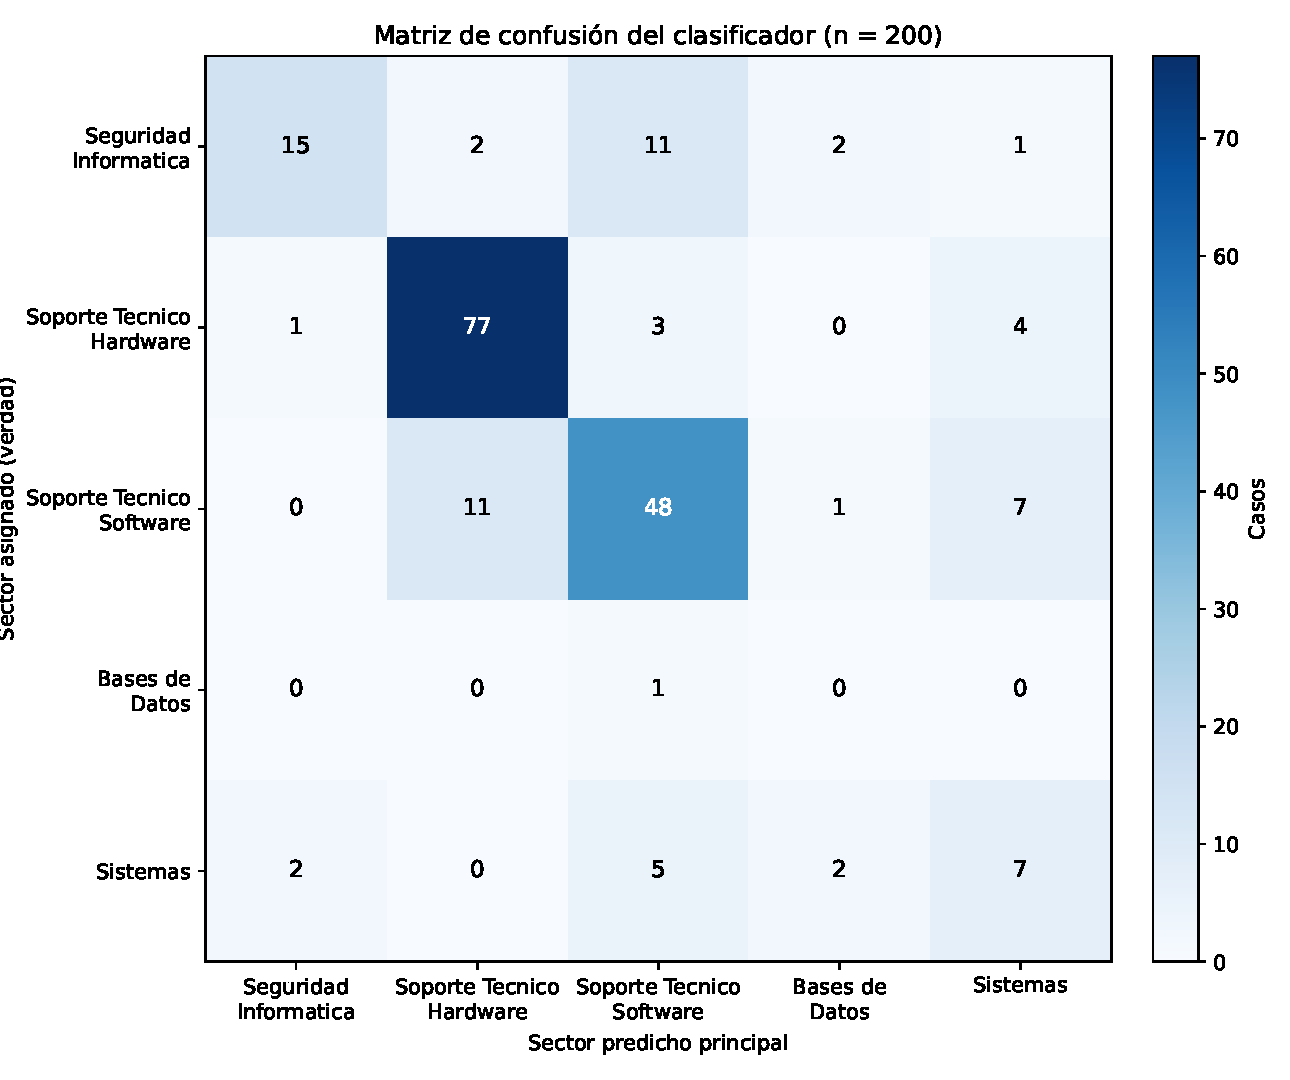
\includegraphics[width=0.85\textwidth]{matriz_confusion}
\caption{Matriz de confusión del clasificador (\(n = 200\)). Filas: sector asignado (verdad); columnas: sector predicho principal.}
\label{fig:matriz_confusion}
\end{figure}

Los valores de precisión, sensibilidad (recall) y F1 por clase, con su intervalo de confianza al 95~\% \parencite{Sokolova2009_performance_measures}, se presentan en la Tabla~\ref{tab:metricas}. La evaluación se enmarca en un único marco métrico cuya referencia de verdad es multietiqueta (107 de los 200 casos, 53,5~\%), frente a una salida del clasificador de una etiqueta principal: la exactitud estricta del 73,5~\% (147/200) es la métrica primaria monoetiqueta, con IC de Wilson al 95~\% de [67,0~\%, 79,1~\%]. El macro-F1 de umbral se reporta sobre las cuatro clases estimables (0,6508), excluida Bases de Datos (\(n = 1\), no estimable), y el de cinco clases (0,5207) se conserva como valor informativo. Las métricas secundarias se calculan contra el conjunto de verdad del corpus (multietiqueta): subset accuracy 0,43 (IC [0,36; 0,50]), Hamming loss 0,3586 (IC [0,31; 0,41]) y micro-F1 0,6654 (IC [0,62; 0,71]). Estas métricas de conjunto penalizan estructuralmente una salida forzada a una sola etiqueta y no son equivalentes de la exactitud estricta: el micro-F1 acumula los aciertos por etiqueta y no por caso, de modo que su valor (0,6654) no debe leerse como una exactitud (0,7350). De los 200 casos, 131 fueron resueltos por la etapa determinística del clasificador y 69 requirieron la etapa Gemini.

\begin{table}[htbp]
\centering
\caption{Métricas de clasificación por clase con intervalo de confianza al 95~\% (una contra el resto)}
\label{tab:metricas}
\small
\setlength{\tabcolsep}{4pt}
\begin{tabular}{@{}>{\raggedright\arraybackslash}p{4.5cm} >{\centering\arraybackslash}p{3.4cm} >{\centering\arraybackslash}p{3.4cm} >{\centering\arraybackslash}p{3.4cm}@{}}
\toprule
\textbf{Clase} & \textbf{Precisión (IC 95~\%)} & \textbf{Sensibilidad (IC 95~\%)} & \textbf{F1 (IC 95~\%)} \\
\midrule
Soporte Tecnico Hardware  & 0,8556 [0,77; 0,91] & 0,9059 [0,83; 0,95] & 0,8800 [0,82; 0,93] \\
Soporte Tecnico Software  & 0,7059 [0,59; 0,80] & 0,7164 [0,60; 0,81] & 0,7111 [0,61; 0,80] \\
Seguridad Informatica     & 0,8333 [0,61; 0,94] & 0,4839 [0,32; 0,65] & 0,6122 [0,44; 0,75] \\
Sistemas                  & 0,3684 [0,19; 0,59] & 0,4375 [0,23; 0,67] & 0,4000 [0,16; 0,59] \\
Bases de Datos            & \multicolumn{3}{c}{no estimable (\(n = 1\))} \\
\bottomrule
\end{tabular}
\par\smallskip
{\footnotesize\textit{Fuente:} elaboración propia a partir del corpus de validación (\(n = 200\)). IC de precisión y sensibilidad por Wilson; IC de F1 por bootstrap percentil (2000 remuestreos).\par}
\end{table}

Estas métricas confirman un desempeño desigual entre las clases objetivo \parencite{Sokolova2009_performance_measures}. Este desequilibrio importa en el contexto operativo, porque un clasificador que concentra sus errores en una clase minoritaria genera derivaciones erroneas en un sector específico y puede erosionar la confianza de ese equipo en la herramienta, independientemente de sus métricas agregadas.

La inspección de la matriz de confusión revela que los 53 errores totales se concentran en fronteras entre sectores léxicamente próximos, con Soporte Tecnico Software como categoría central; su análisis cualitativo, agrupado por frontera de confusión, se desarrolla en la \autoref{subsec:analisis-errores}.

\subsection{Intervención humana en el flujo automatizado}\label{subsec:reduccion-intervencion}

La intervención humana en el flujo automatizado se deriva del gate de revisión implementado, \texttt{requiere\_revision\_humana = (confianza < 0,70)}, que escala un caso a un operador humano cuando la confianza devuelta por el clasificador cae por debajo de ese umbral. El gate de revisión no derivó ningún caso del corpus: la etapa determinística fija el campo en \texttt{False} y la etapa Gemini nunca devolvió una confianza inferior a 0,85.

La sub-hipótesis de intervención humana por caso se declara no contrastada por ausencia de registro primario: la proporción no se computa como resultado, de modo que el aporte operativo asociado al gate queda, por lo tanto, como no medido.

\subsection{Calibración de la confianza}
\label{subsec:calibracion}

La confianza declarada por el clasificador solo resulta útil como criterio de derivación si guarda relación con la exactitud real. Para verificar esa relación se contrastó, sobre los 200 casos del corpus, la confianza devuelta en cada predicción contra la corrección de la clasificación. La Tabla~\ref{tab:bandas} desagrega la exactitud por bandas de confianza en torno al umbral del 70~\% que gobierna el gate de revisión humana.

\begin{table}[htbp]
\centering
\caption{Exactitud por banda de confianza declarada}
\label{tab:bandas}
\small
\begin{tabular}{@{}l c c c@{}}
\toprule
\textbf{Banda de confianza} & \textbf{Casos} & \textbf{Aciertos} & \textbf{Exactitud} \\
\midrule
\([0{,}00\,;\,0{,}50)\) & 98 & 75 & 0,765 \\
\([0{,}50\,;\,0{,}70)\) & 26 & 19 & 0,731 \\
\([0{,}70\,;\,0{,}85)\) & 6  & 2  & 0,333 \\
\([0{,}85\,;\,0{,}95)\) & 31 & 22 & 0,710 \\
\([0{,}95\,;\,1{,}00]\) & 39 & 29 & 0,744 \\
\bottomrule
\end{tabular}
\par\smallskip
{\footnotesize\textit{Fuente:} elaboración propia a partir del corpus de validación (\(n = 200\)).\par}
\end{table}

Los datos revelan una calibración invertida o anti-calibrada: los casos de confianza alta (\(\ge 0{,}70\)) fueron menos exactos (0,697) que los de confianza baja (\(< 0{,}70\), 0,758). La tendencia se acentúa en el extremo superior de la escala: dentro de los 46 casos con confianza igual o superior a 0,90 se registraron 13 errores (28,3~\%), y la banda \([0{,}70\,;\,0{,}85)\) alcanzó apenas 0,333 de exactitud. En otras palabras, el clasificador no solo no discrimina mejor cuando declara mayor certeza, sino que en los tramos de confianza más alta la exactitud se degrada. La consecuencia operativa es directa: el gate del 70~\% no aisló los errores, porque estos se distribuyen también en las bandas de confianza alta. Este hallazgo fundamenta la discusión de la \autoref{sec:discusion}.

\subsection{Análisis de errores y casos límite}\label{subsec:analisis-errores}

El análisis cualitativo de los 53 casos mal clasificados permitió identificar patrones de error recurrentes, agrupados por frontera de confusión y sintetizados en la Tabla~\ref{tab:errores}.

\begin{table}[htbp]
\centering
\caption{Confusiones observadas en la clasificación automática, por frontera}
\label{tab:errores}
\small
\begin{tabular}{@{}>{\raggedright\arraybackslash}p{8.5cm} p{2.0cm} p{2.5cm}@{}}
\toprule
\textbf{Frontera de confusión} & \textbf{Casos} & \textbf{Proporción} \\
\midrule
Soporte Tecnico Hardware \(\leftrightarrow\) Soporte Tecnico Software & 14 & 26,4~\% \\
Sistemas \(\leftrightarrow\) Soporte Tecnico Software & 12 & 22,6~\% \\
Seguridad Informatica \(\leftrightarrow\) Soporte Tecnico Software & 11 & 20,8~\% \\
Otras fronteras & 16 & 30,2~\% \\
\midrule
\textbf{Total} & \textbf{53} & \textbf{100~\%} \\
\bottomrule
\end{tabular}
\par\smallskip
{\footnotesize\textit{Fuente:} elaboración propia a partir del corpus de validación (\(n = 200\)).\par}
\end{table}

El patrón dominante, presente en 14 casos (26,4~\% de los errores), corresponde a la frontera entre Soporte Tecnico Hardware y Soporte Tecnico Software: incidentes en que una falla física de un equipo afecta a una aplicación, o en que una tarea sobre una aplicación se describe con términos de equipamiento, de modo que la decisión correcta depende del juicio humano sobre que aspecto prevalece. El segundo patrón, presente en 12 casos (22,6~\%), corresponde a la frontera entre Sistemas y Soporte Tecnico Software, asociada a acciones sobre servidores y servicios de plataforma descritas como problemas de una aplicación. El tercer patrón, presente en 11 casos (20,8~\%), corresponde a la frontera entre Seguridad Informatica y Soporte Tecnico Software, vinculada a incidentes de acceso y credenciales. El 30,2~\% restante se reparte entre las demas fronteras, incluidas las confusiones que involucran a Bases de Datos, con un único caso de soporte.

Los patrones anteriores se ilustran con tres casos mal clasificados del corpus. Las descripciones se reproducen pseudonimizadas y se acompañan con el sector asignado, el sector predicho y la confianza declarada por el clasificador. El primer caso corresponde al patrón de descripción corta: la entrada ``No puede ingresar al sistema central'' fue asignada a Seguridad Informatica y predicha como Soporte Tecnico Software con una confianza de 0,95; su brevedad no aporta contexto sobre el recurso ni sobre la naturaleza del acceso fallido, de modo que la frontera resulta indistinguible sin información adicional. El segundo ilustra la mezcla de categorías: ``Su equipo se reinicia de forma reiterada; el usuario sospecha de los cables'' fue asignada a Soporte Tecnico Software y predicha como Soporte Tecnico Hardware con 0,50 de confianza, y combina un síntoma de nivel de aplicación con una hipótesis de causa física cuyo peso relativo no queda determinado por el texto. El tercero ejemplifica la jerga local: ``No le salen los correos por el flujo interno y no le llegan las instancias'' fue asignada a Sistemas y predicha como Soporte Tecnico Software con 0,85 de confianza, y apela a términos organizacionales (``flujo'', ``instancias'') cuyo significado no está disponible para el clasificador. En los tres casos la confianza declarada es alta pese al error.

\newpage
